\documentclass[12pt,letterpaper]{article}
\usepackage[utf8]{inputenc}
\usepackage{kpfonts}
\usepackage[T1]{fontenc}

\usepackage{titlesec}

\titlespacing*\section{0pt}{12pt plus 4pt minus 2pt}{0pt plus 2pt minus 2pt}
\titlespacing*\subsection{0pt}{12pt plus 4pt minus 2pt}{0pt plus 2pt minus 2pt}
\titlespacing*\subsubsection{0pt}{12pt plus 4pt minus 2pt}{0pt plus 2pt minus 2pt}

% Package for double spacing
\usepackage{setspace}

% Set 1.0 inch margins
\usepackage[margin=1.0in, headheight=15pt]{geometry}

% Use images and graphics
\usepackage{graphicx}
\usepackage{float}

% Use nicer headers
\usepackage{fancyhdr}
\pagestyle{fancy}
\renewcommand{\headrulewidth}{0pt}
\rhead{CIS3750 - Assignment 1}

% sections should be indexed with alphabets
\renewcommand{\thesection}{\Alph{section}}
\doublespacing

\title{Assignment 1}

\begin{document}
\begin{titlepage}
    \centering
    \vspace*{\baselineskip}
    \rule{\textwidth}{1.6pt}\vspace*{-\baselineskip}\vspace*{2pt}
    \rule{\textwidth}{0.4pt}\\[1.5\baselineskip]
    {\LARGE \textsc{An Initial Outline of a Software System to Improve Food Security in Malawi}}\\[\baselineskip]
	\rule{\textwidth}{0.4pt}\vspace*{-\baselineskip}\vspace{4pt}    
    \rule{\textwidth}{2pt}\\[2\baselineskip]
   
    \vspace*{5\baselineskip}
    \textsc{BY}\\[0.25\baselineskip]
    {\LARGE HANLON} \\
    
    \vspace*{\baselineskip}
    % List of authors in alphabetical order (by last name)
    {\textsc{David DiMaria \\ Braydon Johnson \\ Joshua Lemieux \\ Neivin Mathew \\ Like Zheng} \par}
    \vfill
    {\scshape September 30, 2016} \\
  \end{titlepage}
  
  
% Table of Contents (no page numbers on contents)
\pagenumbering{roman} %roman numerals for ToC
\tableofcontents
\lhead{} % remove default header from Contents page
\clearpage
\pagenumbering{arabic} %pagenumbering in arabic numbers
    
\section{Client Details}
Malawi is a country located in the warm heart of Africa, with a population of 16.4 million. Last year, there were 1 million people in Malawi facing a problem known as food insecurity. This year, that number will rise to 6.4 million. The economy of the country is based on agriculture. Most of the people in Malawi are farmers who grow tobacco for living. Due to the impact of climate change and the growing lack of food, the farmers need to transition to growing different crops. The problem is that many of the Malawians have never grown anything besides tobacco, and do not contain the knowledge to start growing other crops. This is the issue that ARET are trying to solve. \par

ARET (Agricultural Research and Extension Trust) is a research organization in Malawi. They are Malawi’s premier research institution, which are  responsible for conducting research and providing technical/extension services on tobacco. The Trust was established on September 1st, 1995 to foster development and information dissemination for Malawi’s tobacco industry. It amalgamated the services of two institutions, Tobacco Research Institute of Malawi (TRIM) and the Estate Extension Service Trust (EEST), who separately provided research and extension services respectively (reference 1). \par

ARET states their vision as “To be a leading regional centre of excellence in agricultural research and technology dissemination which promotes diversification in the agricultural sector.” (ARET Strategic Plan 2016-2021). 

\clearpage
\section{Team Details}
\subsection{Team Name and Logo}
The team name for the project is "Hanlon."\par
The name is inspired by the eponymous highway that runs through the city of Guelph, and signifies the team's ties to the University of Guelph, as well as the city of Guelph.\\

\begin{figure}[H]
	\centering	
	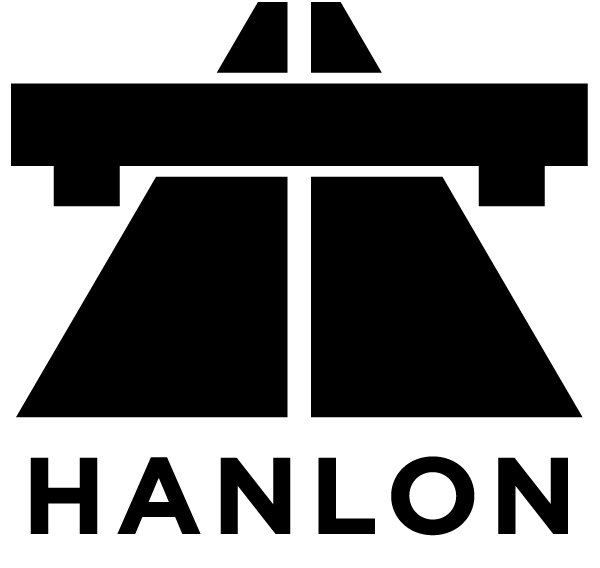
\includegraphics[height=2in]{img/hanlon-logo.png}
	%\caption{The team logo}
	\label{fig:kitten}
\end{figure}

\subsection{Team Members}
Hanlon is comprised of the following students:\\
1. \textbf{\hspace*{5pt} David DiMaria} - Project Manager\\
2. \textbf{\hspace*{5pt}Braydon Johnson} - Software Developer, User Interface Designer\\
3. \textbf{\hspace*{5pt}Joshua Lemieux} - Project Manager, User Interface Designer\\
4. \textbf{\hspace*{5pt}Neivin Mathew} - Software Developer, User Interface Designer\\
5. \textbf{\hspace*{5pt}Like Zheng} - Software Developer

\subsection{Team Roles}
\subsubsection*{Project Manager}
The Project Manager predicts potential problems that may arise during development, and plans tasks to ensure that the project is completed successfully and on time. This role involves the scheduling and unblocking of tasks. It may also involve some programming.

\subsubsection*{Software Developer}
The Developer is involved in all aspects of the software development process including research, design, coding, documentation and testing.

\subsubsection*{User Interface Designer}
The User Interface (UI) Designer role is to plan out and develop any user facing component of the system which includes the specific layout of screens, and improving the interaction between the customer and the product.

\subsection{Team Organization}
Hanlon will follow a static team structure. Each member will maintain their respective roles for the entire duration of the project. \par

Hanlon will use a democratic majority voting system for any decisions that need to be taken within the team. Each present member will be involved in voting, and possesses one vote per motion. A motion is passed when a simple majority is achieved. \par

In the event of a team member being unavailable, and a majority cannot be established, a motion can only be passed through unanimous consent.

\clearpage
\section{Project Goals and Users}
\subsection{Project Goals}

The goal of the project is to design and develop a system that allows the Agricultural Research and Extension Trust (ARET) of Malawi to provide agricultural information to the farmers of Malawi, and relay the data collected from the system back to ARET and its partners.

\subsection{Users}
1.\hspace*{5pt} \textbf{System Administrator -- } Maintains database and API.\\
2.\hspace*{5pt} \textbf{Researcher -- } Creates research materials and reviews extension materials. \\
3.\hspace*{5pt} \textbf{Extension Service --} Creates resources for farmers from research materials. \\
4.\hspace*{5pt} \textbf{Extension Officer -- } Acts as the liaison between the Researcher and Extension Agent \\
5.\hspace*{5pt} \textbf{Extension Agent -- } Acts as the liaison between the Extension Officer and the Farmer. \\
6.\hspace*{5pt} \textbf{Farmer -- } Views information resources , supplies farm data, and responds to surveys. \\
7.\hspace*{5pt} \textbf{Partner -- } Collaborates with ARET, and may access the database and web portal \\
8.\hspace*{5pt} \textbf{Public -- } Uses the system without a user account. Includes any individual that does not fit into the other user groups. \\
9.\hspace*{5pt} \textbf{System -- } Consists of the entire platform (web, mobile), database, and API.

\subsection{Project Organization}
Version control of the codebase will be done using Git. Trello will be used to keep track of sprints and other project management tasks. Communication within the team and between teams will be accomplished through Slack.\par
The database will be built with SQL, using MySQL or PostgreSQL. The API would be developed in Python on the Django REST Framework. The web portal and mobile application will be built concurrently using HTML5, CSS3, and JavaScript, while relying on the Adobe PhoneGap framework to create a hybrid platform.

\clearpage
\section{Requirements}
\subsection{Definitions}
The terms used in the requirements document are defined as follows:\\
1. \hspace*{5pt} \textbf{ARET -- } The Agricultural Research and Extension Trust of Malawi. \\
2. \hspace*{5pt} \textbf{SMS -- } Short Message Service. A service on cell phones that allows the exchange of short text messages.\\
3. \hspace*{5pt} \textbf{API -- } Application Programming Interface. A set of tools that allows applications to interact with each other.\\
4. \hspace*{5pt} \textbf{SQL -- } Structured Query Language. A language that allows the definition and manipulation of data.\\
5. \hspace*{5pt} \textbf{GUI -- } Graphical User Interface. A visual framework that enables easy interaction with an application.

\subsection{Requirements Table}
The table of requirements can be found as a .csv file attached to the report.

\clearpage
\section{Individual Contributions}
\subsection{Josh Lemieux}
\textbf{Collaboration is the New Competitive Advantage}\par
I'm going to be honest, after reading the articles provided and actually thinking about an answer to the question, I could not think of a single thing that I was passionate about that would truly help people. It was honestly a little bit of a shocker. It's not that there was nothing I was passionate about, there would be plenty of technologies I would love to work on and companies I would love to work for. But none of them were really solving important issues, and that was a little depressing. So I decided to analyze my life and some of the things I may take for granted. I realized something in that second, I was sitting in a Starbucks drinking a ridiculously overpriced fancy latte. I thought\ldots here I am drinking a \$5 drink when millions of people in developing countries are just wishing for a little bit of fresh water.\par
So I wondered how much water could be bought with just \$5? I came across an article (Marc Montgomery, rcient 2016) that shocked me.\par
The article states that Nestle pays less than \$5 per million litres of water removed. So, for the price of my one \$5 latte, Nestle could give a litre of fresh water to a million people. That is simply astonishing. I don't think I really need to explain how important it is to have fresh water, but if you're up for a challenge just avoid drinking anything for a full 24 hours, you will soon realize how bad being dehydrated can be.\par
Now what would I do if I had practically infinite funds? I would simply buy a few companies like Nestle and stop worrying about having the perfect profit margins and start worrying about my fellow mankind. The most depressing part is, even with the changes I would make the company would likely still be profitable. So why not now?



\clearpage
\subsection{David DiMaria}
\textbf{Collaboration is the New Competitive Advantage}

After reading the articles provided, there was a lot to think about in regards to how I am going to use my degree after I graduate. Obviously I’d like to be employed by a software company, and make good money. However, I hadn’t given much thought to where I would want to work within computer science, and whether or not it was important that I’m passionate about what I’m working on professionally. If I could use my skills towards some world challenge, it would be the right to knowledge, and specifically the right to free internet. To elaborate on that, I grew up in the age where by the time I was able to type, search engines were extremely popular and any information that I wanted was right at my fingertips. I could know anything at any moment, uncensored, as long as I had a stable internet connection. I could learn about anything I want, immerse myself in online communities, share information with my peers and find like minded individuals from all around the world.\par

This is a challenge since a large portion of the world doesn’t have internet access, and many that do have portions censored based on which country they're from. This is something that people should care about because if impoverished people can learn anything at any moment, they could be saved from governments trying to suppress them physically and intellectually. The reason why governments will try and censor things is because of the amount of political unrest it would cause given there people had all the information. The power that information could have on a population is unfathomable, because they could learn the truth about how their government is perceived in the eyes of the rest of the world.\par

If I could choose a group of people to help me achieve this goal, it would be Google, Facebook, and telecommunications companies. The power of internet infrastructure at companies like Google and Facebook is large enough that they could develop a worldwide satellite network with telecommunications companies that delivers internet to everyone.

\clearpage
\subsection{Like Zheng}
\textbf{What is the Real Challenge?}\par
After I read the two articles, I still think we are making the world better. Everyone’s behaviour is changing the world. Small steps can make significant changes. \par
Someone may say, “Not everyone is doing useful things, or solving real problems.” What is a real issue? I can’t say “a service that delivers your beer right to your door” is not solving real problems. People can use this time to do other things instead of buying a beer. Also, it is a real job to someone. The world is how it looks like it is. People are doing trivial things for a reason. Maybe they don’t want to go out, so there are delivery services; they feel loose, so there is an app to help you understand “cause and effect in their life.”; Cars pollute the Earth, so there is an electric car. It is the fact that nobody can say it is wrong or not before actually doing it.\par
I thought about it for a few minutes. What do I want to do and what is the challenge I interested? Usually, I may say, “I want to make a fancy game or app everybody want to use.” However, for now, I feel I never know what I want to do unless I tried everything. Thus, I decide to try more things I never tried before.\par
After all, if I can have all money in the world, I can hire all experts from every domain, and talk with them. So I can have their specialized opinion to see different point of views. 

\clearpage
\subsection{Neivin Mathew}
\textbf{The Advancement of Prosthetics}\par
One billion people, about fifteen percent of the world's population, live with some kind of disability. While any kind of disability has the potential to be debilitating, a physical disability is certainly the most crippling. Persons with physical disabilities are statistically more likely to experience worse socio-economic conditions than those without a disability. They suffer from poorer education, lower employment rates, and greater levels of poverty.\par
Improving the lives of a huge part of the global population is not only a noble endeavour, but has numerous benefits such as increasing a country's workforce and GDP, and a rise in the overall quality of life. However, physical disabilities are the hardest disabilities to treat. In many cases, such as when an individual has lost a limb or some other vital organ, a cure is simply impossible. In these situations, the best we can do is mitigate the effects of the disability with crude prosthetics.\par
Most prosthetics available today are still very primitive. Although research is being done on more advanced robotic prosthetics, there are a huge economic or geographic barriers restricting access to these technologies. The greatest challenge prosthetics and other disability aids face is how expensive they are to develop and build. Another issue is that how unique every individual's disability is, thus many prosthetics need to be custom made for each patient. \par
Having unlimited finds would open many doors in the advancement of prosthetics. Collaboration from fields such as neuroscience, kinesiology, mechanical engineering, and computing would help the technology grow in leaps and bounds.


\clearpage
\subsection{Braydon Johnson}
\textbf{The Problem with Today's Education System}\par
The challenge that is of particular interest to me is how the public education system in Canada (and other countries) is currently structured and how it is failing. Children are expected to conform to standard style of teaching and their abilities are assessed via standardized tests designed by some board of education. With the advancements in research on education that we have seen just in the last twenty years that show children do not all learn the same way or test the same way, it is absurd that the educational system is reluctant to change the way it educates children, both in style of teaching and the teachers in which they employ.\par
Teachers have one of the largest impacts on a child's life outside of the home and some of them are just terrible people and terrible teachers in general,  but there is not a lot to be done about them because of things like tenure and the Teacher's Union. I have personal experience with this because the public school in my home town became a dumping ground for problematic teachers that could not be fired so they were placed somewhere that the Board of Education believed they would cause the least amount of damage. My education from grade one to grade five consisted teachers that couldn't care less about the students they were teaching and whose ability to teach was severely lacking.\par
If I had all the money in the world I would attempt to create a way to help students get in contact with educators that could best serve their educational needs rather than having to gamble with the public education system. To make this endeavour a reality I would bring together Teachers, Parents, Researchers from many different disciplines and Computer Scientists.

\end{document}